\section{Results}
\label{sec:results}

In this section, we present the results of each research question.

\subsection{RQ1: How  is the {\tt re} module used in Python projects?}
To address this research question, we look at regex utilizations, flags, and the most frequently observed pattern strings.

\subsubsection{Regex Utilizations per Project}
Out of the \DTLfetch{data}{key}{nProjScanned}{value}\ projects scanned, \DTLfetch{data}{key}{percentProjectsUsingRegex}{value}\% (\DTLfetch{data}{key}{nProjectsUsingRegex}{value}) contained at least one regex utilization.  For context about how saturated these projects were with utilizations, we consider how many utilizations were observed per project, how many files the average scanned project  contained, how many of those files contained utilizations, and how many utilizations occurred per file, as shown in Table~\ref{table:saturation}.

The average project contained 32 utilizations, and the maximum number of utilizations was 1,427.  The project with the most utilizations is a C\# project\footnote{\url{https://github.com/Ouroboros/Arianrhod}} that maintains a collection of source code for 20 Python libraries, including larger libraries like {\tt pip}, {\tt celery} and {\tt ipython}.  These larger Python libraries contain many utilizations.

% to find max nprojects: select distinct uniqueSourceID, count(*) as ct from RegexCitationMerged group by uniqueSourceID order by ct;


From Table~\ref{table:saturation}, we also see that each project had an average of 11 files containing any utilization, and each of these files had an average of 2 utilizations.  As we scanned \DTLfetch{data}{key}{nProjScanned}{value} projects, we would expect to have seen $11*2*3898=85,756$ regex usages, which is higher than the actual \DTLfetch{data}{key}{nUsages}{value} usages observed. \todo{Explain why? Be pedantic. }

\begin{table}[tb]
\begin{center}
\begin{small}
\caption{How saturated are projects with utilizations? (RQ2)}
\label{table:saturation}

\begin{tabular}{l|ccccc}
\toprule
source & Q1 & Avg & Med & Q3 & Max \\ 
 \hline \bigstrut
utilizations per project & 2 & 32 & 5 & 19 & 1,427 \\ 
 \hline \bigstrut
files per project & 2 & 53 & 6 & 21 & 5,963 \\ 
 \hline \bigstrut
utilizing files per project & 1 & 11 & 2 & 6 & 541 \\ 
 \hline \bigstrut
utilizations per file & 1 & 2 & 1 & 3 & 207 \\ 
\bottomrule
\end{tabular}
\end{small}
\end{center}
\end{table}


\subsubsection{Usage Frequency of {\tt re} Module Functions}

\begin{figure}[tb]
\centering
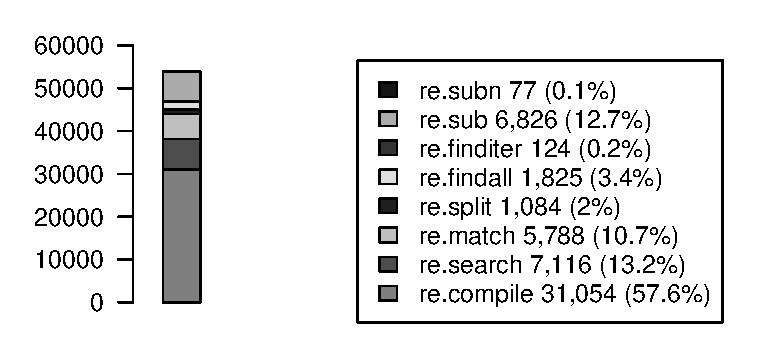
\includegraphics[width=\columnwidth]{../analysis_output/partFunctions.eps}
\caption{How often are the 8 re functions used? (RQ1)}
\label{fig:partFunctions}
\end{figure}

\begin{figure}[tb]
\centering
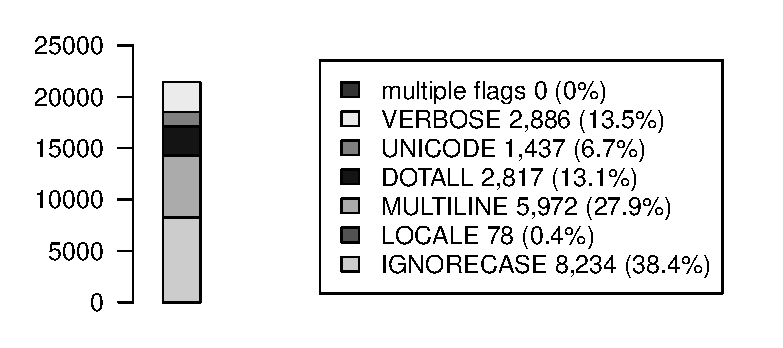
\includegraphics[width=\columnwidth]{../analysis_output/partFlags.eps}
\caption{Which behavioral flags are used? (RQ1)}
\label{fig:partFlags}
\end{figure}

The number of projects that use each of the {\tt re} functions are shown in Figure~\ref{fig:partFunctions}.  The y-axis denotes the total utilizations, with a maximum of \DTLfetch{data}{key}{nUsages}{value}. The {\tt re.compile} function encompasses \DTLfetch{data}{key}{percentCompile}{value}\% of all utilizations, presumably because each usage of those functions can accept a regex object compiled using {\tt re.compile} as an argument.

\subsubsection{Usage Frequency of {\tt re} Module Flags}
When considering flag use, we excluded the default flag, which is built into the {\tt re} module, and present internally whenever no flag is used.  Of all utlizations, \DTLfetch{data}{key}{percentFlags0}{value}\% had no flag, or explicitly specified the default flag (which is equivalent).  The debug flag, which causes the {\tt re} regex engine to display extra information about its parsing process, was never observed. \todo{interesting about the debug flag. Any idea why?}

 Figure~\ref{fig:partFlags} presents the number of projects in which each flag appears. \todo{the numbers in the key do not appear to sum to the max on the Y-axis of this figure} Of all behavioral flags used, ignorecase (\DTLfetch{data}{key}{percentI}{value}\%) and multiline (\DTLfetch{data}{key}{percentM}{value}\%) were the most frequently used.  It is also worth noting that although multiple flags can be combined using a bitwise or, this was never observed.


\subsubsection{Most Frequently Observed Patterns}

Table~\ref{table:topNW} contains the most frequently used patterns, ordered by the number of projects that the pattern appears in.  The patterns are quoted to show the presence of spaces, if any.  For brevity, we will only elaborate on the top four patterns, and we will reference the feature set in Table~\ref{table:featureStats}, as described in Section~\ref{results:re2}.

The first pattern, \verb!`\s+'!, uses the WSP character class feature.  This character class represents one or more whitespace characters,  defined as spaces, tabs, newlines, vertical whitespace, carriage returns or form feeds.  The \verb!+! (the ADD feature) at the end of the pattern means that it must match one or more whitespace characters.  The pattern \verb!`\s+'! is often used to split sentences into separate words which may have more than one space between them, or contain tabs or other types of whitespace.

Interestingly, the second most common pattern, \verb!`\s'!, also uses the WSP character. In this case, it does not match several whitespace characters (though it would match the first of several).

The third pattern, \verb!\d+!,  uses the DEC character class, which is composed of the digits from 0 to 9.  Like the first pattern, the third uses the ADD feature to match one or more digits.

The fourth pattern, \verb![\x80-\xff]!, uses the CCC feature to create a custom character class, and the RNG feature to specify a range of characters.
%The hexadecimal value \verb!\x80! is equivalent to the value 128 in decimal, and the hexadecimal value \verb!\xff! is equivalent to 255 in decimal.
When hexadecimal values are used within a character class like this (and the UNICODE flag is not active), it signifies the corresponding characters in an ASCII lookup table.
%The range specified by this pattern is highlighted on the right side of Figure~\ref{fig:ASCIItable}.  Table image found at: \url{https://courses.engr.illinois.edu/ece390/books/labmanual/ascii-code/quickref.png}.
%\todo{run program again to unescape pattern strings}
%\todo{Figure 6 seems largely unnecessary}


%\todo{more of the topN patterns if there is space}

%\begin{figure}[tb]
%\centering
%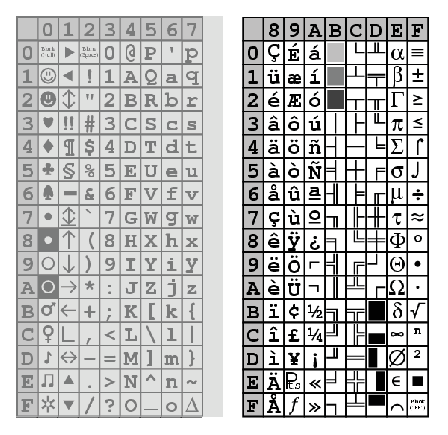
\includegraphics[width=\columnwidth]{../illustrations/ASCIItable.eps}
%\cprotect\caption{On the Right, ASCII Characters Matching \verb!'[\x80-\xff]'! (RQ1)}
%\label{fig:ASCIItable}
%\end{figure}

\begin{table}
\caption{ \label{}}
\begin{center}
\begin{tabular}{lc}
\toprule
pattern & weight \\ 
\midrule
\begin{minipage}{2.3in}
\begin{verbatim}
'\\s+'\end{verbatim}
\end{minipage}
& 181 \\ 
\midrule
\begin{minipage}{2.3in}
\begin{verbatim}
'\\s'\end{verbatim}
\end{minipage}
& 78 \\ 
\midrule
\begin{minipage}{2.3in}
\begin{verbatim}
'\\d+'\end{verbatim}
\end{minipage}
& 70 \\ 
\midrule
\begin{minipage}{2.3in}
\begin{verbatim}
'[\\x80-\\xff]'\end{verbatim}
\end{minipage}
& 69 \\ 
\midrule
\begin{minipage}{2.3in}
\begin{verbatim}
'\nmd5_data = {\n([^}]+)}'\end{verbatim}
\end{minipage}
& 69 \\ 
\midrule
\begin{minipage}{2.3in}
\begin{verbatim}
'\\\\(.)'\end{verbatim}
\end{minipage}
& 67 \\ 
\midrule
\begin{minipage}{2.3in}
\begin{verbatim}
'([\\\\"]|[^\\ -~])'\end{verbatim}
\end{minipage}
& 66 \\ 
\midrule
\begin{minipage}{2.3in}
\begin{verbatim}
'(-?(?:0|[1-9]\\d*))(\\.\\d+)?([eE][-+]?\\d+)?'\end{verbatim}
\end{minipage}
& 61 \\ 
\midrule
\begin{minipage}{2.3in}
\begin{verbatim}
'[^]]+?\\] +([0-9.]+): (\\w+) <-(\\w+)'\end{verbatim}
\end{minipage}
& 60 \\ 
\midrule
\begin{minipage}{2.3in}
\begin{verbatim}
'.*rlen=([0-9]+)'\end{verbatim}
\end{minipage}
& 57 \\ 
\bottomrule
\end{tabular}
\end{center}
\end{table}


% %\subsection{Pattern Characteristics}

% Table~\ref{table:patternStats} (description of table contents)

% \begin{table}[tb]
\begin{center}
\caption{Pattern Characteristics (RQ1)}
\label{table:patternStats}

\begin{tabular}{l|ccccc}
\toprule
source & Q1 & Avg & Med & Q3 & Max \\ 
\midrule
pattern weight & 1 & 2 & 1 & 2 & 182 \\ 
\midrule
token count & 8 & 23 & 14 & 24 & 31,349 \\ 
\midrule
distinct features & 3 & 5 & 5 & 7 & 20 \\ 
\midrule
pattern length & 13 & 37 & 22 & 38 & 43,255 \\ 
\bottomrule
\end{tabular}
\end{center}
\end{table}

\todo{add patternStats table back in and describe it if there is enough time.  Note the longest pattern present in patternLength.csv in analysis folder was probably automatially generated from text and is monstrous!}


\subsubsection{Summary of Results for RQ1}
Only about half of the projects sampled contained any utilizations, and many of these utilizations came from python module source code that had been copied into projects, not code written by the users.  Most utilizations used the {\tt re.compile} function to compile a regex object before actually using the regex to find a match.  Most utilizations did not use a flag to modify matching behavior.  The most frequently observed patterns were used to match whitespace and digits.

\subsection{RQ2: Which regular expression language features are most commonly used in python?}
\label{results:re2}

Table~\ref{table:featureStats} displays feature usage from the corpus and relates it to four major regex related projects. Only features appearing in at least 10 projects are listed.
The first column, \emph{rank}, lists the rank of a feature (relative to other features) in terms of the number of projects in which it appears. The next column, \emph{code}, gives a succinct reference string for the feature, and is followed by a \emph{description} column that provides a brief comment on what the feature does.  The \emph{example} column provides a short example of how the feature can be used.
% For example, the most common feature observed in the corpus is \emph{one-or-more repetition}, which is specified in a pattern by using the {\tt +} character in conjunction with some sub-pattern that should repeat one or more times.  The code for this feature is \emph{ADD}, and the short example provided is \verb!z+!.
The next four columns map to the four major research projects chosen for our investigation (see Section~\ref{results:rq3}).  We indicate that a project supports a feature with the `\yes' symbol, and indicate that a project does not support the feature with the `\no' symbol.

The next six columns contain three pairs of usage statistics.  The first pair contains the number and percent of \emph{patterns} that a feature appears in, out of the 13,912 patterns that make up the corpus. The next pair of columns contain the number and percent of \emph{files} that a feature appears in out of the 18,549 files scanned that contain at least one utilization.  The last pair of columns contain the number and percent of \emph{projects} that a feature appears in out of the 1645 projects scanned that contain at least one utilization.

One notable omission from Table~\ref{table:featureStats} is the literal feature, which is used  to specify matching any specific character.  An example pattern that contains only one literal token is the pattern \verb!`a'!.  This pattern only matches the lowercase letter `a'.  The literal feature was found in \DTLfetch{data}{key}{P_LITERAL_PRESENT}{value}\% of patterns.
%, and accounted for \DTLfetch{data}{key}{P_LITERAL_TOKENS}{value}\% of all tokens.
We consider the literal feature to be ubiquitous in all patterns, and necessary for any regex related tool to support, and so exclude it from Table~\ref{table:featureStats} and the rest of the feature analysis.


\subsubsection{Feature Usage}
The eight most commonly used features, ADD, CG, KLE, CCC, ANY, RNG, STR and END,
appear in over half the projects. The remaining 26 features appear in less than half of the projects containing utilizations.

%The seven most rarely used features,  LKB, ENDZ, BKR, NDEC, BKRN, VWSP and NWNW, appear in fewer than 8.  These seven features are more rarely used than all other features with respect to all three of our usage statistics.  Less than 8\% of scanned projects containing utilizations contain these features.
%removed because this table is not complete - features in less than 10 projects are omitted so talking about the least used is not entirely accurate

%\subsubsection{Potentially Under-Ranked and Over-Ranked Features}
Table~\ref{table:featureStats} is sorted by the number of projects a feature appears in, but if the table were instead sorted by the number of patterns or files that a feature appears in, the ranking order would be different.  CG is more commonly used in patterns than the highest ranked feature (ADD) by a wide margin (over 8\%).  CG is also more commonly used with respect to how many files it appears in by 2.3\%, while only being present in 12 fewer projects (0.7\%) than ADD.

The WSP feature is present in more patterns than the NCCC feature by a margin of 6.7\%, and in more files by a margin of 4.2\%, yet it is ranked lower than NCCC because it is present in 13 fewer projects (0.8\%).
The WNW, OPT and QST features follow the same pattern of being under-ranked in terms of the number of patterns and files that they appear in.



\subsubsection{Feature Support in Regex Projects}
Of the four projects selected for analysis, RE2 supports the most features (28 features) followed by hampi (25 features),  Rex (21 features), and brics (12 features).  All projects support the 8 most commonly used features except brics, which does not support STR or END.  All projects support NCC, OR, and the four less common repetition features: QST, SNG, DBB and LWB.

No projects support the four look-around features LKA, NLKA, LKB and NLKB.  RE2 and hampi support the LZY, NCG, PNG and OPT features, whereas brics and Rex do not.  Brics is the only project that does not support any of the six default character classes (WSP, DEC, WRD, NWSP, NWRD, NDEC) - the rest of the projects support all of those features.  RE2 is the only project to support the WNW, ENDZ and NWNW features.  RE2 also supports the PNG feature (which allows you to name capturing groups), but does not support the BKRN feature which is necessary to refer back to the named capture group.

\begin{table*}[h]
\begin{center}
\begin{small}
\caption{How Frequently do Features Appear in Projects? (RQ2)}
\label{table:featureStats}
\begin{tabular}
{ll@{ }llc@{ }c@{ }c@{ }ccccccc}
rank & code & description & example & brics & hampi & Rex & RE2 & nPatterns & \% patterns & nProjects & \% projects \\ 
\toprule[0.16em]
1 & ADD & one-or-more repetition & \begin{minipage}{0.5in}\begin{verbatim}z+\end{verbatim}\end{minipage} & \yes & \yes & \yes & \yes & 6,003 & 44.1 & 1,204 & 73.2 \\ 
\midrule
2 & CG & a capture group & \begin{minipage}{0.5in}\begin{verbatim}(caught)\end{verbatim}\end{minipage} & \yes & \yes & \yes & \yes & 7,130 & 52.4 & 1,194 & 72.6 \\ 
\midrule
3 & KLE & zero-or-more repetition & \begin{minipage}{0.5in}\begin{verbatim}.*\end{verbatim}\end{minipage} & \yes & \yes & \yes & \yes & 6,017 & 44.3 & 1,099 & 66.8 \\ 
\midrule
4 & CCC & custom character class & \begin{minipage}{0.5in}\begin{verbatim}[aeiou]\end{verbatim}\end{minipage} & \yes & \yes & \yes & \yes & 4,468 & 32.9 & 1,026 & 62.4 \\ 
\midrule
5 & ANY & any non-newline char & \begin{minipage}{0.5in}\begin{verbatim}.\end{verbatim}\end{minipage} & \yes & \yes & \yes & \yes & 4,657 & 34.3 & 1,005 & 61.1 \\ 
\midrule
6 & RNG & chars within a range & \begin{minipage}{0.5in}\begin{verbatim}[a-z]\end{verbatim}\end{minipage} & \yes & \yes & \yes & \yes & 2,631 & 19.3 & 848 & 51.6 \\ 
\midrule
7 & STR & start-of-line & \begin{minipage}{0.5in}\begin{verbatim}^\end{verbatim}\end{minipage} & \no & \yes & \yes & \yes & 3,563 & 26.2 & 846 & 51.4 \\ 
\midrule
8 & END & end-of-line & \begin{minipage}{0.5in}\begin{verbatim}$\end{verbatim}\end{minipage} & \no & \yes & \yes & \yes & 3,169 & 23.3 & 827 & 50.3 \\ 
\midrule[0.12em]
9 & NCCC & negated CCC & \begin{minipage}{0.5in}\begin{verbatim}[^qwxf]\end{verbatim}\end{minipage} & \yes & \yes & \yes & \yes & 1,935 & 14.2 & 776 & 47.2 \\ 
\midrule
10 & WSP & \textbackslash t \textbackslash n \textbackslash r \textbackslash v \textbackslash f or space & \begin{minipage}{0.5in}\begin{verbatim}\s\end{verbatim}\end{minipage} & \no & \yes & \yes & \yes & 2,846 & 20.9 & 762 & 46.3 \\ 
\midrule
11 & OR & logical or & \begin{minipage}{0.5in}\begin{verbatim}a|b\end{verbatim}\end{minipage} & \yes & \yes & \yes & \yes & 2,102 & 15.5 & 708 & 43 \\ 
\midrule
12 & DEC & any of: 0123456789 & \begin{minipage}{0.5in}\begin{verbatim}\d\end{verbatim}\end{minipage} & \no & \yes & \yes & \yes & 2,297 & 16.9 & 692 & 42.1 \\ 
\midrule
13 & WRD & [a-zA-Z0-9\_] & \begin{minipage}{0.5in}\begin{verbatim}\w\end{verbatim}\end{minipage} & \no & \yes & \yes & \yes & 1,430 & 10.5 & 650 & 39.5 \\ 
\midrule
14 & QST & zero-or-one repetition & \begin{minipage}{0.5in}\begin{verbatim}z?\end{verbatim}\end{minipage} & \yes & \yes & \yes & \yes & 1,871 & 13.8 & 645 & 39.2 \\ 
\midrule
15 & LZY & as few reps as possible & \begin{minipage}{0.5in}\begin{verbatim}z+?\end{verbatim}\end{minipage} & \no & \yes & \no & \yes & 1,300 & 9.6 & 605 & 36.8 \\ 
\midrule
16 & NCG & group without capturing & \begin{minipage}{0.5in}\begin{verbatim}a(?:b)c\end{verbatim}\end{minipage} & \no & \yes & \no & \yes & 791 & 5.8 & 404 & 24.6 \\ 
\midrule
17 & PNG & named capture group & \begin{minipage}{0.5in}\begin{verbatim}(?P<name>x)\end{verbatim}\end{minipage} & \no & \yes & \no & \yes & 915 & 6.7 & 354 & 21.5 \\ 
\midrule
18 & SNG & exactly n repetition & \begin{minipage}{0.5in}\begin{verbatim}z{8}\end{verbatim}\end{minipage} & \yes & \yes & \yes & \yes & 581 & 4.3 & 340 & 20.7 \\ 
\midrule
19 & NWSP & any non-whitespace & \begin{minipage}{0.5in}\begin{verbatim}\S\end{verbatim}\end{minipage} & \no & \yes & \yes & \yes & 484 & 3.6 & 270 & 16.4 \\ 
\midrule
20 & DBB & $n\le x \le m$ repetition & \begin{minipage}{0.5in}\begin{verbatim}z{3,8}\end{verbatim}\end{minipage} & \yes & \yes & \yes & \yes & 367 & 2.7 & 238 & 14.5 \\ 
\midrule
21 & NLKA & sequence doesn't follow  & \begin{minipage}{0.5in}\begin{verbatim}a(?!yz)\end{verbatim}\end{minipage} & \no & \no & \no & \no & 131 & 1 & 183 & 11.1 \\ 
\midrule
22 & WNW & word/non-word boundary & \begin{minipage}{0.5in}\begin{verbatim}\b\end{verbatim}\end{minipage} & \no & \no & \no & \yes & 248 & 1.8 & 166 & 10.1 \\ 
\midrule
23 & NWRD & non-word chars & \begin{minipage}{0.5in}\begin{verbatim}\W\end{verbatim}\end{minipage} & \no & \yes & \yes & \yes & 94 & 0.7 & 165 & 10 \\ 
\midrule
24 & LWB & at least n repetition & \begin{minipage}{0.5in}\begin{verbatim}z{15,}\end{verbatim}\end{minipage} & \yes & \yes & \yes & \yes & 91 & 0.7 & 158 & 9.6 \\ 
\midrule
25 & LKA & matching sequence follows & \begin{minipage}{0.5in}\begin{verbatim}a(?=bc)\end{verbatim}\end{minipage} & \no & \no & \no & \no & 112 & 0.8 & 158 & 9.6 \\ 
\midrule
26 & OPT & options wrapper & \begin{minipage}{0.5in}\begin{verbatim}(?i)CasE\end{verbatim}\end{minipage} & \no & \yes & \no & \yes & 231 & 1.7 & 154 & 9.4 \\ 
\midrule
27 & NLKB & sequence doesn't precede & \begin{minipage}{0.5in}\begin{verbatim}(?<!x)yz\end{verbatim}\end{minipage} & \no & \no & \no & \no & 94 & 0.7 & 137 & 8.3 \\ 
\midrule[0.12em]
28 & LKB & matching sequence precedes & \begin{minipage}{0.5in}\begin{verbatim}(?<=a)bc\end{verbatim}\end{minipage} & \no & \no & \no & \no & 80 & 0.6 & 120 & 7.3 \\ 
\midrule
29 & ENDZ & absolute end of string & \begin{minipage}{0.5in}\begin{verbatim}\Z\end{verbatim}\end{minipage} & \no & \no & \no & \yes & 89 & 0.7 & 90 & 5.5 \\ 
\midrule
30 & BKR & match the $i^{th}$ CG & \begin{minipage}{0.5in}\begin{verbatim}\1\end{verbatim}\end{minipage} & \no & \no & \no & \no & 60 & 0.4 & 84 & 5.1 \\ 
\midrule
31 & NDEC & any non-decimal & \begin{minipage}{0.5in}\begin{verbatim}\D\end{verbatim}\end{minipage} & \no & \yes & \yes & \yes & 36 & 0.3 & 58 & 3.5 \\ 
\midrule
32 & BKRN & references PNG & \begin{minipage}{0.5in}\begin{verbatim}\g<name>\end{verbatim}\end{minipage} & \no & \yes & \no & \no & 17 & 0.1 & 28 & 1.7 \\ 
\midrule
33 & VWSP & matches U+000B & \begin{minipage}{0.5in}\begin{verbatim}\v\end{verbatim}\end{minipage} & \no & \no & \yes & \yes & 13 & 0.1 & 15 & 0.9 \\ 
\midrule
34 & NWNW & negated WNW & \begin{minipage}{0.5in}\begin{verbatim}\B\end{verbatim}\end{minipage} & \no & \no & \no & \yes & 4 & 0 & 11 & 0.7 \\ 
\bottomrule[0.13em]
\end{tabular}
\end{small}
\end{center}
\vspace{-12pt}
\end{table*}


\subsubsection{Summary of Results for RQ2}
We found that the eight most common features are found on over 50\% of the projects.
%Five features that make more appearances in terms of patterns and files than the feature ranked immediately higher than them in terms of appearances in projects.
We also identify brics as the project supporting the fewest features and RE2 as the project supporting the most features, and identify groups of features supported or not supported by the four regex projects.


\subsection{{RQ3:} What is the impact of \emph{not} supporting various regular expression features on users and tool designers?}
\label{results:rq3}

%\subsubsection{Rationale for Behavioral Clustering}
When tool designers are considering what features to include, data about user behaviors is valuable.  Our clustering technique helps to discern these behaviors by looking beyond the structural details of specific patterns and seeing trends in actual matching behavior.  We are also able to find out what features are being used in these behavioral trends so that we can make assertions about why certain features are important. 

%\subsubsection{General Information About Clusters Found}
From 9503 distinct patterns, the MCL clustering technique identified 514 clusters with 2 or more patterns, and 7214 clusters of size 1.  Recall that only pairs of patterns with a similarity level of \todo{X} were included in the matrix passed to MCL.  The average size of clusters larger than contains 3.7 patterns.
Each pattern belongs to exactly one cluster. 


%\subsubsection{An Example Cluster}
Table~\ref{table:exampleCluster} provides an example of a smaller behavioral cluster, representing 13 patterns, with at least one pattern from this cluster present in 100 different projects.  At first glance this cluster may seem to revolve around the `\verb!\s*!' parts of these patterns, but actually this cluster was formed because each of these patterns has a comma literal, and other details did not interfere with matching the Rex-generated strings with commas in them.

\begin{table}
\begin{center}
\caption{Sample from an example cluster (RQ4)}
\label{table:exampleCluster}
\begin{small}
\begin{tabular}
{lcc | lcc}
\toprule
index & pattern & nProjects & index & pattern & nProjects \\
 \hline \bigstrut
1 & \begin{minipage}{0.3in}\begin{verbatim}`:+'\end{verbatim}\end{minipage} & 8 & 5 & \begin{minipage}{0.5in}\begin{verbatim}`[:]'\end{verbatim}\end{minipage} & 6 \\
 \hline \bigstrut
2 & \begin{minipage}{0.3in}\begin{verbatim}`(:)'\end{verbatim}\end{minipage} & 8 & 6 & \begin{minipage}{0.6in}\begin{verbatim}`([^:]+):(.*)'\end{verbatim}\end{minipage} & 6 \\
 \hline \bigstrut
3 & \begin{minipage}{0.3in}\begin{verbatim}`(:+)'\end{verbatim}\end{minipage} & 8 & 7 & \begin{minipage}{0.5in}\begin{verbatim}`\s*:\s*'\end{verbatim}\end{minipage} & 4 \\
 \hline \bigstrut
4 & \begin{minipage}{0.3in}\begin{verbatim}`(:)(:*)'\end{verbatim}\end{minipage} & 8 & 8 & \begin{minipage}{0.5in}\begin{verbatim}`\:'\end{verbatim}\end{minipage} & 2 \\
\bottomrule
\end{tabular}
\vspace{-6pt}
\end{small}
\end{center}
\end{table}


%
%\begin{table}
%\begin{center}
%\caption{An example cluster (RQ3)}
%\label{table:exampleCluster}
%\begin{small}
%\begin{tabular}
%{lcc}
%\toprule
%index & pattern & nProjects\\
%\midrule
%1 & \begin{minipage}{0.5in}\begin{verbatim}`\s*,\s*'\end{verbatim}\end{minipage} & 54  \\
%\midrule
%2 & \begin{minipage}{0.5in}\begin{verbatim}`,'\end{verbatim}\end{minipage} & 30 \\
%\midrule
%3 & \begin{minipage}{0.5in}\begin{verbatim}`\s*,'\end{verbatim}\end{minipage} & 16 \\
%\midrule
%4 & \begin{minipage}{0.5in}\begin{verbatim}` ,\s*'\end{verbatim}\end{minipage} & 13 \\
%\midrule
%5 & \begin{minipage}{0.5in}\begin{verbatim}` *, *'\end{verbatim}\end{minipage} & 12 \\
%\midrule
%6 & \begin{minipage}{0.5in}\begin{verbatim}`,\S'\end{verbatim}\end{minipage} & 5 \\
%\midrule
%7 & \begin{minipage}{0.5in}\begin{verbatim}`,.*$'\end{verbatim}\end{minipage} & 3 \\
%\midrule
%8 & \begin{minipage}{0.6in}\begin{verbatim}`(\S+)\s*,\s*'\end{verbatim}\end{minipage} & 2 \\
%\midrule
%9 & \begin{minipage}{0.5in}\begin{verbatim}`,+'\end{verbatim}\end{minipage} & 1 \\
%\midrule
%10 & \begin{minipage}{0.5in}\begin{verbatim}`,\ ?'\end{verbatim}\end{minipage} & 1 \\
%\midrule
%10 & \begin{minipage}{0.5in}\begin{verbatim}`,\s*(\S)'\end{verbatim}\end{minipage} & 1 \\
%\midrule
%11 & \begin{minipage}{0.5in}\begin{verbatim}`\s*(,)\s*'\end{verbatim}\end{minipage} & 1 \\
%\midrule
%12 & \begin{minipage}{0.5in}\begin{verbatim}`\s*\,\s*'\end{verbatim}\end{minipage} & 1 \\
%\bottomrule
%\end{tabular}
%\end{small}
%\end{center}
%\end{table}


%\subsubsection{Using the Smallest Pattern to Represent a Cluster}
The smallest pattern in Table~\ref{table:exampleCluster} is the single comma literal \verb!`,'! at index 1.  This smallest pattern gives the a good idea of what all the patterns within it have in common.  A shorter pattern will tend to have less extraneous behavior because it is specifying less behavior.  And yet in order for the smallest pattern to be clustered with other patterns, it had to match most of the {\tt matching\_strings} created by Rex from another pattern within the cluster, and so \emph{the smallest pattern is likely to be sufficient to represent the cluster}.

For the rest of this paper, a cluster will be represented by one of the shortest patterns it contains, followed by the number of projects it appears in, so the cluster in Table~\ref{table:exampleCluster} will be represented as \verb!`,'(100)!.
%The top 10 clusters are shown in Table~\ref{table:topNClusters}, ranked by the number of projects they appear in.
%\subsubsection{Catagorizing the Top 100 Clusters}
We  manually mapped the top 100 clusters into each of 6 behavioral categories, omitting 11 clusters that did not fit into any of these catagories, and 29 clusters composed of long strings (example: \verb!set_fabric_sense_len\)\(!) which were in the top 100 because 28 projects that were scanned were forked linux kernels.


\subsubsection{General Information About Clusters Found}
From 9503 distinct patterns, our clustering technique identified 514 clusters of 2 or more patterns, and 7214 clusters of size 1.  The average size of clusters larger than 1 contains 3.7 patterns.
No two clusters contain the same pattern.


Next, we define the six categories and provide examples from the relevant clusters.  \todo{order the following sub subsections based on popularity}

\subsubsection{Default Character Classes}
This category contains 12 clusters. Each of the clusters \todo{finish this}. For example, three of the top clusters in this category include: 
\verb!`\s'(277)!, \verb!`\W'(208)!, and \verb!`\d'(193)!. 
%\verb!`\w'(114)!, \verb!`\w+$'(71)!, 
% \verb!`\D'(65)!, \verb!`\S'(53)!, \verb!`^\s'(40)!, \verb!`^\d+'(39)!, \verb!`^\s*'(39)!, \verb!`\d+$'(38)!, \verb!`\s*'(30)!

\subsubsection{User-Defined Character Classes}
This category contains 10 clusters. Each of the clusters \todo{finish this}. For example, three of the top clusters in this category include: 
\verb!`[a-zA-Z]'(138)!, \verb•`[^!-~]'(122)•, and \verb!`[&<]'(50)!.
% \verb!`[A-Z]'(47)!, \verb!`[ \t]'(37)!, \verb!`[-\s]'(35)!, \verb!`^[a-zA-Z]'(33)!, \verb!`[][\()<>@,:;"."]'(29)!, \verb!`[*?[]'(29)!, \verb!`[?/]+'(28)!

\subsubsection{Single Literal Characters}
This category contains 19 clusters. Each of the clusters \todo{finish this}. For example, three of the top clusters in this category include: 
\verb!`\\'(110)!, \verb!`,'(100)!, and \verb!`:'(91)!.
% \verb!`-'(74)!, \verb!`#'(69)!, \verb!` '(66)!, \verb!`/'(65)!, \verb!`\.'(61)!, \verb!`='(52)!, \verb!`//'(51)!, \verb!`\n'(41)!, \verb!`;'(38)!, \verb!`_'(36)!, \verb!`@'(36)!, \verb!`"'(33)!, \verb!`%'(29)!, \verb!`&'(28)!, \verb!`&'(28)!, \verb!`''(28)!

\subsubsection{Parsing Variable Assignments}
This category contains 4 clusters. Each of the clusters \todo{finish this}. For example, three of the top clusters in this category include: 
\verb!`\nmd5_data = {\n([^}]+)}'(69)!, \verb!`.*rlen=([0-9]+)'(57)!, and \verb!`coding[:=]\s*([-\w.]+)'(48)!.
%, \verb!`((^|;)\s*charset=)([^;]*)'(34)!

\subsubsection{Parsing Bracket Contents}
This category contains 5 clusters. Each of the clusters \todo{finish this}. For example, three of the top clusters in this category include: 
\verb!`<.+>'(63)!, \verb!`<([^>]*)>: \[0x([0-9a-f]+)-0x([0-9a-f]+)\]'(57)!, and \verb!`(<[^<>]*)/>'(35)!. %, \verb•`<!\s+([^<>]*)>'(35)•,  \verb!`\(.*\)'(31)!

\subsubsection{ Matching Whole Lines}
This category contains 8 clusters. Each of the clusters \todo{finish this}. For example, three of the top clusters in this category include: 
\verb!`^\d+$'(78)!, \verb!`^\w+$'(74)!, and \verb!`^\s*$'(59)!.
%, \verb!`^[-\w]+$'(45)!, \verb!`^[a-zA-Z]\w*$'(43)!, \verb!`^[ ]*(#.*)?$'(41)!, \verb!`^[a-f0-9]{40}$'(34)!, \verb!`^\S+@[a-zA-Z0-9._-]+\.[a-zA-Z0-9._-]+$'(29)!


%\subsubsection{Clusters Not Falling Into Any Category}
%\verb!`\d+\.\d+'(53)!, \verb!`\d+\.\d+\.\d+'(48)!, \verb!`".*"'(42)!,\verb!`*$'(42)!, \verb!`(^|.*:)\s*\w*("|\')'(41)!, \verb!`\(\*'(38)!, \verb!`/|-'(36)!, \verb!`.'(35)!, \verb!`\\|/'(31)!, \verb!`::'(30)!, \verb!`/\*'(29)!

\subsubsection{Summary of Results for RQ3}
We used the behavior of individual patterns to form clusters, and identified six main categories that clusters belonged to.  Overall, we see that many clusters are defined by the presence of particular tokens, such as the comma for the cluster in Table~\ref{table:exampleCluster}.
These six categories define what users are doing with regexes at a high level: using default character classes, defining their own character classes, matching single characters, parsing variable assignments, parsing the contents of brackets, or matching whole lines.
 One of the six common cluster categories, \emph{parsing variable assignments}, has a very specific purpose of parsing source code files. This shows a very specific and common use of regular expressions in practice. 

%whereas each group in the second part is drawn from a subset of strings in the corpus known to contain at least one of the desired features.  We did this because the presence of a feature in a pattern can be easily lost





 %All 1375 projects containing at least 1 Rex-Compatible pattern


% We guide the results analysis for this research question based on the features \emph{not} supported by popular regex tools.
% Table~\ref{table:featureStats} shows the mapping from features to regex tools.





% \subsubsection{Feature Groups Overview}
% Instead of analyzing every feature independently, we chose small groups of conceptually related features.  For each of these groups, we selected all clusters that had at least one of the features in at least one pattern within the cluster to form a `feature group'-focused cluster set.

% Table~\ref{table:featureGroups} shows the total number of projects that contain at least one pattern from at least one cluster in the cluster set, and some selected clusters represented by the shortest string in the cluster.  These clusters were selected not because of being within the largest number of projects, but because they illustrate some interesting usage of a feature that will be explored in detail later.

% 
\begin{table*}
\begin{center}
\caption{Feature Groups with Selected Cluster Examples (RQ3)}
\label{table:featureGroups}
\begin{tabular}
{cccc}
index & feature set & nProjects & selected cluster examples (nProjects for that cluster)\\
\toprule

0 & ADD,KLD,QST & 970 & \begin{minipage}{5in}\begin{verbatim}`\W+'(208), `[A-Z]?[:;.A-Z]'(47), `:+'(91), `https?://'(13)\end{verbatim}\end{minipage}\\
\midrule
1 & CCC,NCCC,RNG & 953 & \begin{minipage}{5in}\begin{verbatim}`[0-9]'(193), `[^!-~]'(122), `[aeiou]'(4), `[^\w!#$%&'*+,.:;<=>?^`|~-]'(14)\end{verbatim}\end{minipage}\\
\midrule
2 & CG & 943 & \begin{minipage}{5in}\begin{verbatim}`coding[:=]\s*([-\w.]+)'(48), `<(.*)>'(63), `"(.*)"'(42), `\\(.)'(110s)\end{verbatim}\end{minipage}\\
\midrule
3 & STR,END & 807 & \begin{minipage}{5in}\begin{verbatim}`^\d+$'(78), `^\\s*$'(59), `,.*$'(100), `=.*$'(52), `^(.*)<(.*)>(.*)$'(63), \end{verbatim}\end{minipage}\\
\midrule
4 & ANY & 801 & \begin{minipage}{5in}\begin{verbatim}`\s.*'(277), `(\d+)(.*)'(193), `-.*'(74), `(.)([A-Z])'(47), `<.+>'(63)\end{verbatim}\end{minipage}\\
\midrule
5 & WSP,NWSP & 775 & \begin{minipage}{5in}\begin{verbatim}`\s'(277), `\S'(53), `:\s*'(91), `,\S'(100), `<\\S[^>]*>'(63)\end{verbatim}\end{minipage}\\
\midrule
6 & OR & 759 & \begin{minipage}{5in}\begin{verbatim}`((the|a|an)\\s+)?[0-9]+'(193), `([ ]+_)|(_[ ]+)|([ ]+)'(66), `<.*>|</.*>'(63)\end{verbatim}\end{minipage}\\
\midrule
7 & DEC,NDEC & 622 & \begin{minipage}{5in}\begin{verbatim}`\d'(193), `\D'(65), `\.\d+$'(14), `[^\w\d_]'(208), `(\D)[.]'(61)\end{verbatim}\end{minipage}\\
\midrule
8 & WRD,NWRD & 595 & \begin{minipage}{5in}\begin{verbatim}`\W'(208), `\w'(114), `[a-zA-Z]\w*'(138), `(\w*)=(\w*)'(52), `\\(\W)'(110) \end{verbatim}\end{minipage}\\
\midrule
9 & DBB,LWB,SNG & 459 & \begin{minipage}{5in}\begin{verbatim}`^[0-9]{1,5}$'(78), `\d{2}'(193), `[.]{2,}'(21), `^[0-9A-Za-z._-]{0,100}$'(27)\end{verbatim}\end{minipage}\\
\bottomrule
\end{tabular}
\end{center}
\end{table*}




% (note that for the ANY group, all but two of the top 30 clusters used `.*', but that .* as a pattern alone only appeared in 23 projects)


% tell them how the cluster groups in the first part are all drawn from a subset of the corpus limited by what Rex can support, whereas the cluster groups in the second part are all drawn from the complete corpus, but are not guaranteed to have behavioral similarity like in the first part.


